

%% AP Physics MC Questions Archive
%%----------------------------------------


%% Kinetic Energy
%%----------------------------------------
\element{ap}{
\begin{question}{kinetic-energy-q01}
    %Base your answer to the following question on the force vs. distance graph below,
    The force vs distance graph below shows an object being pushed along a straight line,
        starting from rest.
    \begin{center}
    \begin{tikzpicture}
        \begin{axis}[
            axis y line=left,
            axis x line=bottom,
            axis line style={->},
            xlabel={distance},
            x unit=\si{\meter},
            xtick={0,2,4,6},
            minor x tick num=1,
            ylabel={force},
            y unit=\si{\newton},
            ytick={0,5,10,15,20},
            minor y tick num=1,
            xmin=0,xmax=6.2,
            ymin=0,ymax=22,
            grid=major,
            width=0.8\columnwidth,
            height=0.5\columnwidth,
        ]
        \addplot[line width=1pt,mark=\empty] plot coordinates {(0,10) (2,0) (3,20) (6,20)};
        \end{axis}
    \end{tikzpicture}
    \end{center}
    If the object has a mass of \SI{1.4}{\kilo\gram},
        what is its velocity at \SI{5.0}{\meter}?
    \begin{multicols}{3}
    \begin{choices}
        \wrongchoice{\SI{0.2}{\meter\per\second}}
        \wrongchoice{\SI{2.0}{\meter\per\second}}
        \wrongchoice{\SI{5.0}{\meter\per\second}}
      \correctchoice{\SI{9.25}{\meter\per\second}}
        \wrongchoice{\SI{15}{\meter\per\second}}
    \end{choices}
    \end{multicols}
\end{question}
}

\element{ap}{
\begin{question}{kinetic-energy-q02}
    A particle is fired straight up out of a cannon.
    Which of the following graphs best represents its kinetic energy as a function of time?
    \begin{multicols}{2}
    \begin{choices}
        \AMCboxDimensions{down=-2.5em}
        \wrongchoice{
            \begin{tikzpicture}
                \begin{axis}[
                    axis y line=left,
                    axis x line=bottom,
                    axis line style={->},
                    xlabel={time},
                    xtick=\empty,
                    ylabel={energy},
                    ytick=\empty,
                    xmin=0,xmax=11,
                    ymin=0,ymax=11,
                    width=0.95\columnwidth,
                ]
                \addplot[line width=1pt,domain=0:10]{0.4*x*(x-10)};
                \end{axis}
            \end{tikzpicture}
        }
        \wrongchoice{
            \begin{tikzpicture}
                \begin{axis}[
                    axis y line=left,
                    axis x line=bottom,
                    axis line style={->},
                    xlabel={time},
                    xtick=\empty,
                    ylabel={energy},
                    ytick=\empty,
                    xmin=0,xmax=11,
                    ymin=0,ymax=11,
                    width=0.95\columnwidth,
                ]
                \addplot[line width=1pt,domain=0:10]{10-0.32*(x-5)*(x-5)};
                \end{axis}
            \end{tikzpicture}
        }
        %% ANS is C
        \correctchoice{
            \begin{tikzpicture}
                \begin{axis}[
                    axis y line=left,
                    axis x line=bottom,
                    axis line style={->},
                    xlabel={time},
                    xtick=\empty,
                    ylabel={energy},
                    ytick=\empty,
                    xmin=0,xmax=11,
                    ymin=0,ymax=11,
                    width=0.95\columnwidth,
                ]
                \addplot[line width=1pt,domain=0:10]{0.32*(x-5)*(x-5)};
                \end{axis}
            \end{tikzpicture}
        }
        \wrongchoice{
            \begin{tikzpicture}
                \begin{axis}[
                    axis y line=left,
                    axis x line=bottom,
                    axis line style={->},
                    xlabel={time},
                    xtick=\empty,
                    ylabel={energy},
                    ytick=\empty,
                    xmin=0,xmax=11,
                    ymin=0,ymax=11,
                    width=0.95\columnwidth,
                ]
                \addplot[line width=1pt,domain=0:10]{2+0.32*(x-5)*(x-5)};
                \end{axis}
            \end{tikzpicture}
        }
        \wrongchoice{
            \begin{tikzpicture}
                \begin{axis}[
                    axis y line=left,
                    axis x line=bottom,
                    axis line style={->},
                    xlabel={time},
                    xtick=\empty,
                    ylabel={energy},
                    ytick=\empty,
                    xmin=0,xmax=11,
                    ymin=0,ymax=11,
                    width=0.95\columnwidth,
                ]
                \addplot[line width=1pt,domain=0:10]{8};
                \end{axis}
            \end{tikzpicture}
        }
    \end{choices}
    \end{multicols}
\end{question}
}

\element{ap}{
\begin{question}{kinetic-energy-q03}
    A block of mass $m$ moving with initial velocity $v_0$ moves over a rough surface with coefficient of kinetic friction $\mu$.
    How long does it take for the block to come to a complete stop?
    \begin{multicols}{3}
    \begin{choices}
        \wrongchoice{$\dfrac{v_0^2}{2\mu g}$}
        \wrongchoice{$\dfrac{v_0^2}{2m\mu g}$}
        \wrongchoice{$\dfrac{v_0^2}{\mu g}$}
        \wrongchoice{$\dfrac{v_0}{2\mu g}$}
      \correctchoice{$\dfrac{v_0}{\mu g}$}
    \end{choices}
    \end{multicols}
\end{question}
}

\element{ap}{
\begin{question}{kinetic-energy-q04}
    %Base your answer to the following question on
    The picture below represents a plane \SI{10}{\meter} in length with a coefficient of kinetic friction of \num{0.2},
        inclined at an angle of \ang{53}.
    A block of weight \SI{30}{\newton} is placed at the top of the plane and allowed to slide down.
    \begin{center}
    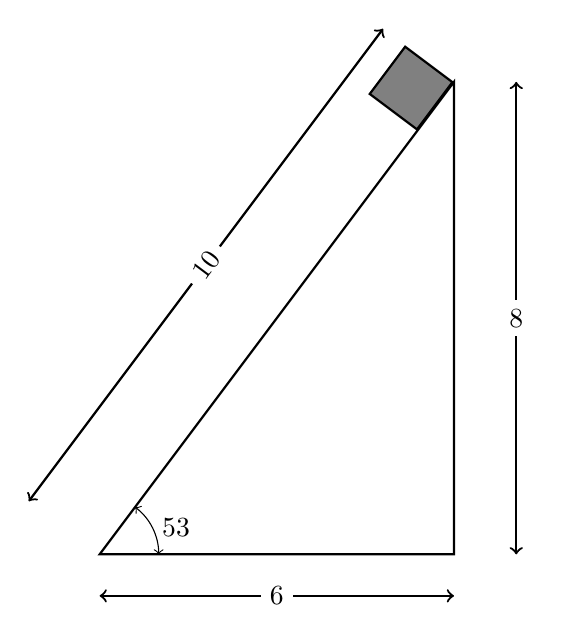
\begin{tikzpicture}[scale=0.75]
        %% Triangle
        \draw[thick] (0,0) -- (6,0) -- (6,8) -- cycle;
        %% Labels
        \draw[<->] (1,0) arc (0:53.13:1) node[pos=0.5,anchor=west] {\ang{53}};
        \draw[<->,thick] (0,-2em) -- (6,-2em) node[pos=0.5,anchor=center,fill=white] {\SI{6}{\meter}};
        \draw[<->,thick] (6cm+3em,0) -- (6cm+3em,8) node[pos=0.5,anchor=center,fill=white] {\SI{8}{\meter}};
        \draw[<->,thick] (143.13:1.5) -- ++(53.13:10) node[pos=0.5,anchor=center,rotate=53.13,fill=white] {\SI{10}{\meter}};
        %% block
        \node[draw,thick,minimum size=0.75cm,fill=white!50!black,rotate=53.13,anchor=south east] (A) at (53.13:10cm) {};
    \end{tikzpicture}
    \end{center}
    The velocity of the block after its \SI{10}{\meter} slide down the plane is most nearly:
    \begin{multicols}{3}
    \begin{choices}
        %% NOTE: correct answer is 11.55 m/s
      \correctchoice{\SI{11.5}{\meter\per\second}}
        \wrongchoice{\SI{8.2}{\meter\per\second}}
        \wrongchoice{\SI{8.6}{\meter\per\second}}
        \wrongchoice{\SI{8.9}{\meter\per\second}}
        \wrongchoice{\SI{9.7}{\meter\per\second}}
        \wrongchoice{\SI{10.0}{\meter\per\second}}
    \end{choices}
    \end{multicols}
\end{question}
}

\element{ap}{
\begin{question}{kinetic-energy-q05}
    %% Base your answer to the following question on the following information.
    A proton weighing \SI{1.67e-27}{\kilo\gram} is accelerated from rest for a time of \SI{e-8}{\second} by a uniform electric field that exerts a force of \SI{6.4e-14}{\newton} on the proton.
    %% Start question
    The distance over which the proton accelerated is most nearly:
    \begin{multicols}{2}
    \begin{choices}
        \wrongchoice{\SI{2.0e-7}{\meter}}
        \wrongchoice{\SI{2.0e-5}{\meter}}
      \correctchoice{\SI{2.0e-3}{\meter}}
        \wrongchoice{\SI{2.0e-1}{\meter}}
        \wrongchoice{\SI{2.0e0}{\meter}}
    \end{choices}
    \end{multicols}
\end{question}
}

\element{ap}{
\begin{question}{kinetic-energy-q06}
    An object at rest weighs \SI{100}{\newton} on earth.
    It gains \SI{100}{\joule} of kinetic energy.
    What is its velocity?
    \begin{multicols}{2}
    \begin{choices}
        \wrongchoice{$\sqrt{10}\,\si{\meter\per\second}$}
        \wrongchoice{$\sqrt{15}\,\si{\meter\per\second}$}
      \correctchoice{$\sqrt{20}\,\si{\meter\per\second}$}
        \wrongchoice{$\sqrt{25}\,\si{\meter\per\second}$}
        \wrongchoice{$\sqrt{30}\,\si{\meter\per\second}$}
    \end{choices}
    \end{multicols}
\end{question}
}

\element{ap}{
\begin{question}{kinetic-energy-q07}
    A car with kinetic energy \SI{20 000}{\joule} travels along a horizontal road.
    How much work is required to stop the car in \SI{5}{\second}?
    \begin{multicols}{3}
    \begin{choices}
        \wrongchoice{\SI{0}{\joule}}
      \correctchoice{\SI{20 000}{\joule}}
        \wrongchoice{\SI{4 000}{\joule}}
        \wrongchoice{\SI{8 000}{\joule}}
        \wrongchoice{\SI{16 000}{\joule}}
    \end{choices}
    \end{multicols}
\end{question}
}

\element{ap}{
\begin{question}{kinetic-energy-q08}
    How much energy is required to stop a car of mass \SI{100}{\kilo\gram} traveling at \SI{25}{\meter\per\second}?
    \begin{multicols}{3}
    \begin{choices}
        \wrongchoice{\SI{1 150}{\joule}}
        \wrongchoice{\SI{21 150}{\joule}}
      \correctchoice{\SI{31 250}{\joule}}
        \wrongchoice{\SI{32 250}{\joule}}
        \wrongchoice{\SI{42 250}{\joule}}
    \end{choices}
    \end{multicols}
\end{question}
}

\element{ap}{
\begin{question}{kinetic-energy-q09}
    Two balls of equal size are dropped from the same height from the roof of a building.
    One ball has mass $M$ and the other has a mass $2M$.
    %% graphic is not needed
    When the balls reach the ground,
        how do the kinetic energies of the two balls compare?
    (Neglect friction)
    \begin{choices}
        \wrongchoice{$M$ has one-fourth the kinetic energy of $2M$.}
      \correctchoice{$M$ has one-half the kinetic energy of $2M$.}
        \wrongchoice{$M$ has the same amount of kinetic energy as $2M$.}
        \wrongchoice{$M$ has twice the amount of kinetic energy as $2M$.}
        \wrongchoice{$M$ has four times the amount of kinetic energy as $2M$.}
    \end{choices}
\end{question}
}

\element{ap}{
\begin{question}{kinetic-energy-q10}
    A rail gun is able to accelerate a projectile with a mass of \SI{4}{\kilo\gram} from rest to \SI{100}{\meter\per\second} in \SI{5}{\second}.
    Calculate the work done on the projectile by the force of the rail gun.
    \begin{multicols}{2}
    \begin{choices}
        \wrongchoice{\SI{1.0e2}{\joule}}
        \wrongchoice{\SI{5.0e2}{\joule}}
      \correctchoice{\SI{2.0e4}{\joule}}
        \wrongchoice{\SI{1.0e5}{\joule}}
        \wrongchoice{Cannot be determined from the information provided.}
    \end{choices}
    \end{multicols}
\end{question}
}

\element{ap}{
\begin{question}{kinetic-energy-q11}
    An object with a mass of \SI{2}{\kilo\gram} increases in speed from \SI{4}{\meter\per\second} to \SI{12}{\meter\per\second} in \SI{3}{\second}.
    The total work performed on the object during this time is:
    \begin{multicols}{3}
    \begin{choices}
        \wrongchoice{\SI{16}{\joule}}
        \wrongchoice{\SI{64}{\joule}}
      \correctchoice{\SI{128}{\joule}}
        \wrongchoice{\SI{256}{\joule}}
        \wrongchoice{\SI{512}{\joule}}
    \end{choices}
    \end{multicols}
\end{question}
}

\element{ap}{
\begin{question}{kinetic-energy-q12}
    A \SI{100}{\watt} motor propels an object with a mass of \SI{4}{\kilo\gram} for \SI{2}{\second} from rest.
    Its final velocity will be:
    \begin{multicols}{3}
    \begin{choices}
        \wrongchoice{\SI{5}{\meter\per\second}}
      \correctchoice{\SI{10}{\meter\per\second}}
        \wrongchoice{\SI{20}{\meter\per\second}}
        \wrongchoice{\SI{40}{\meter\per\second}}
        \wrongchoice{\SI{100}{\meter\per\second}}
    \end{choices}
    \end{multicols}
\end{question}
}

\element{ap}{
\begin{question}{kinetic-energy-q13}
    Which of the following graphs best represents the kinetic energy of a particle as a function of the momentum of the particle?
    \begin{multicols}{2}
    \begin{choices}
        \AMCboxDimensions{down=-2.5em}
        %% ANS is A
        \correctchoice{
            \begin{tikzpicture}
                \begin{axis}[
                    axis y line=left,
                    axis x line=bottom,
                    axis line style={->},
                    xlabel={momentum},
                    xtick=\empty,
                    ylabel={energy},
                    ytick=\empty,
                    xmin=0,xmax=11,
                    ymin=0,ymax=11,
                    width=0.95\columnwidth,
                ]
                \addplot[line width=1pt,domain=0:10]{0.1*x*x};
                \end{axis}
            \end{tikzpicture}
        }
        \wrongchoice{
            \begin{tikzpicture}
                \begin{axis}[
                    axis y line=left,
                    axis x line=bottom,
                    axis line style={->},
                    xlabel={momentum},
                    xtick=\empty,
                    ylabel={energy},
                    ytick=\empty,
                    xmin=0,xmax=11,
                    ymin=0,ymax=11,
                    width=0.95\columnwidth,
                ]
                \addplot[line width=1pt,domain=0:10]{x};
                \end{axis}
            \end{tikzpicture}
        }
        \wrongchoice{
            \begin{tikzpicture}
                \begin{axis}[
                    axis y line=left,
                    axis x line=bottom,
                    axis line style={->},
                    xlabel={momentum},
                    xtick=\empty,
                    ylabel={energy},
                    ytick=\empty,
                    xmin=0,xmax=11,
                    ymin=0,ymax=11,
                    width=0.95\columnwidth,
                ]
                \addplot[line width=1pt,domain=0:10]{10-x};
                \end{axis}
            \end{tikzpicture}
        }
        \wrongchoice{
            \begin{tikzpicture}
                \begin{axis}[
                    axis y line=left,
                    axis x line=bottom,
                    axis line style={->},
                    xlabel={momentum},
                    xtick=\empty,
                    ylabel={energy},
                    ytick=\empty,
                    xmin=0,xmax=11,
                    ymin=0,ymax=11,
                    width=0.95\columnwidth,
                ]
                \addplot[line width=1pt,domain=0:10]{10/x};
                \end{axis}
            \end{tikzpicture}
        }
        %% 5) none of the above
    \end{choices}
    \end{multicols}
\end{question}
}

\element{ap}{
\begin{question}{kinetic-energy-q14}
    A person does \SI{100}{\joule} of work in pulling back the string of a bow.
    What will be the initial speed of a \SI{0.5}{\kilo\gram} arrow when it is fired from the bow?
    \begin{multicols}{3}
    \begin{choices}
      \correctchoice{\SI{20}{\meter\per\second}}
        \wrongchoice{\SI{50}{\meter\per\second}}
        \wrongchoice{\SI{200}{\meter\per\second}}
        \wrongchoice{\SI{400}{\meter\per\second}}
        \wrongchoice{\SI{800}{\meter\per\second}}
    \end{choices}
    \end{multicols}
\end{question}
}

\element{ap}{
\begin{question}{kinetic-energy-q15}
    If an object sliding on a rough surface experiences an increase in kinetic energy of $E$ while it is pushed by a constant force $F$ through a distance $d$,
        what is the force due to friction?
    \begin{multicols}{3}
    \begin{choices}
        \wrongchoice{$Fd - E$}
      \correctchoice{$\dfrac{Fd - E}{d}$}
        \wrongchoice{$\dfrac{F-E}{d}$}
        \wrongchoice{$Fd $}
        \wrongchoice{$\dfrac{E}{d} - F$}
    \end{choices}
    \end{multicols}
\end{question}
}

\element{ap}{
\begin{question}{kinetic-energy-q16}
    What happens to the energy of a bouncing ball as it hits the ground with a certain downward velocity?
    \begin{choices}
        \wrongchoice{Gravitational Potential energy is converted into kinetic energy.}
        \wrongchoice{Elastic Potential Energy is converted into gravitational potential energy}
        \wrongchoice{Kinetic energy is converted into heat energy.}
      \correctchoice{Kinetic energy is converted into elastic potential energy and heat.}
        \wrongchoice{Kinetic energy is converted into gravitational energy.}
    \end{choices}
\end{question}
}

\element{ap}{
\begin{question}{kinetic-energy-q17}
    Which of the following is true of a \SI{1}{\kilo\gram} mass and a \SI{5}{\kilo\gram} mass that both fall from rest from the same height?
    \begin{choices}
        \wrongchoice{the force felt due to gravity is the same on both masses}
        \wrongchoice{their initial potential energies are equal}
        \wrongchoice{they lose potential energy at the same rate}
        \wrongchoice{they have the same kinetic energy upon hitting the ground}
      \correctchoice{their accelerations are equal}
    \end{choices}
\end{question}
}


\endinput


